%%%%%%%%%%%%%%%%%%%%%%%%%%%%%%%%%%%%%%%%%%%%%%%%%%%%%%%%%%%%%%%%%%%%%%%%%%%%%%%%
\Chapter{Introduction}{}{}
\label{ch:intro}
\glsresetall
%%%%%%%%%%%%%%%%%%%%%%%%%%%%%%%%%%%%%%%%%%%%%%%%%%%%%%%%%%%%%%%%%%%%%%%%%%%%%%%% 
% 
The power grid represents one of the major backbones of the human civilization.
It determines our supply chain, which includes important infrastructures such as
water supply and heating. \textcite{Els17} gives an impression---although
fictional---of how essential the power grid is and which parts of our daily life
are actually affected by a blackout. However, to sustain the basic human needs
we have to change towards a more sustainable and environmentally friendly
behavior in general and in power grids in particular. Thus, the future power
grid has to become more efficient to handle the increasing demand for energy as
well as the planned increasing number of generators that transform renewable
energies~\parencite{online:eeg2014}, \eg, wind into electrical energy. We call
these generators \emph{renewable energy producers}. Renewable energy producers
such as wind turbines are~\acrlong{ipp} (\gls{ipp}) that have a volatile power
production pattern---meaning that the amount of production is influenced by many
uncertainties such as the weather---that is totally different
from~\emph{conventional power generators} (\eg, nuclear and coal power plants),
where the production is stable.

The power grid has evolved historically and the traditional structure
interconnects few central conventional power generators with many consumers
(\cref{ch:intro:fig:power-grid-structure} left side) in such a way that the
demand of the consumers is always satisfied. Similar to the road network, where
we distinguish roads by their speed limits and size into rural roads, highways,
and motorways, we are able to distinguish the lines in the power grid depending
on the amount of power they are able to transfer. The power grid's hierarchical
structure in Germany consists of high (\SI{110}{\glssymbol{kv}}, \SI{220}{
\glssymbol{kv}}, and~\SI{380}{\glssymbol{kv}}), medium ($1$
to~$50$~\glssymbol{kv}), and low voltage layers (\SI{230}{\glssymbol{volt}}
and~\SI{400}{\glssymbol{volt}}; see~\cref{ch:intro:fig:power-grid-structure})
representing transmission and distribution power grids, respectively. In a
conventional power grid the power producers are connected to the high voltage
layer directly and the consumers are either connected to the medium voltage
layer (\eg, industries), or low voltage layer (\eg, households and small
industries). Within this hierarchical structure the power grid consists of edges
that are represented by power lines or cables that interconnect producers with
consumers. These edges are often denoted as elements (or branches) as they could
also represent power electronics such as transformers, resistors, and
conductors.
%  
\begin{figure}[t!]
    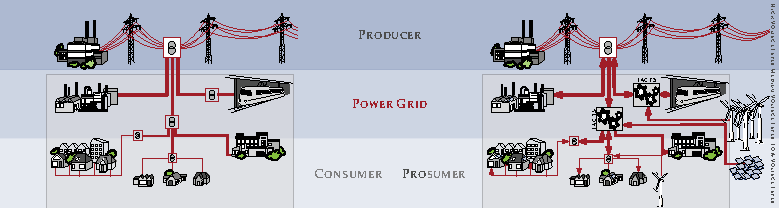
\includegraphics{intro/fig/power-grid-structure.pdf}%
    % 
    \caption[Change of the power grid hierarchical structure.]{Two exemplary
    power grids showing the conventional power grid (left) and the current
    development of the power grid (right). Both power grids consists of three
    voltage layers. On the~\myhl{KITseablue50}{high voltage layer} there are the
    conventional power plants (\eg, coal and nuclear power plants) as well as
    bigger collections of wind farms and~\acrlong{vpp}s located. The industrial
    consumers are usually located on the~\myhl{KITseablue30}{medium voltage
    layer} that mainly presents a distribution layer. In
    the~\myhl{KITseablue15}{low voltage layer}, we have the households and small
    industrial consumers. Note that on the right side, participants of the last
    two layer might have photovoltaics and wind turbines and are thus denoted by
    the term \emph{prosumers} (\ie, acting as producer and consumer
    simultaneously).%
    }%
    % 
    \label{ch:intro:fig:power-grid-structure}%
\end{figure} 

Renewable energy producers are often added to the medium and low voltage layer
(\cref{ch:intro:fig:power-grid-structure} right side). This eventually causes a
bidirectional power flow which the conventional power grid was not designed for.
This change in the power grid usage might cause instabilities and new critical
lines. Critical lines represent lines, which removal might cause a blackout. The
idea of the latter problem is exemplary shown in~\parencite{Wit16}. Offshore
wind farms in the North and Baltic Sea
(see~\cref{ch:intro:fig:north-sea-wind-farms}) provide another example for such
producers. In this particular case, the suitability of a location for such farms
highly depends on the wind profile and available space. Thus, the location for
wind farms is not as flexible as for conventional power plants. These offshore
wind farms produce---similar to conventional power plants---a high amount of
electrical energy that is not used on-site. However, it is largely required in
areas such as the Ruhr region, and southern regions of
Germany~\parencite{online:europe:project132:hvdc-line-a-north,online:europe:project235:HVDC_SuedLink_Brunsbuettel_Wilster-to-Grossgartach_Grafenrheinfeld,online:europe:TYNDP-2018-Projects-Sheets-166,online:europe:north-south-interconnections},
since a large number of industrial consumers are located there. Sending such an
amount of energy through the power grid causes new bottlenecks or is simply
impossible. Switching these wind farms off to sustain the grid safety is not a
desirable solution. Thus, to cope with these new challenges
the~\acrlong{tso}~(\gls{tso}) can follow at least two possible strategies.
% 
\crefformat{enumi}{#2\textup{Strategy~#1}#3}
\begin{enumerate}[(S1)]
    % 
    \item The expansion of the power grid by adding new transmission lines and
    \label{ch:intro:strategy:1}
    % 
    \item the installation of advanced control units such as~\acrlong{facts} 
    (\gls{facts}) and switches for a better utilization of the existing power
    grid.
    \label{ch:intro:strategy:2}
    % 
\end{enumerate}
% 
The mentioned power grid structure and strategies lead to the~\emph{dynamic}
and~\emph{static transmission design problem}~\parencite{Bin01a}.
\textcite{Bin01a} consider~\cref{ch:intro:strategy:1} as dynamic transmission
design problems~\parencite{Gal92,Cho06,Bin01a} under which long-term power
grid configuration such as~\acrlong{tnep} (\gls{tnep}) is encountered.
\gls{tnep}~\parencite{Hem13} is the design problem of adding new 
transmission lines or circuits under different objectives such as the cost
minimization of the new added transmission lines or maximization of the
throughput of the power grid. Adding new transmission lines decreases the total
power grid resistance~\parencite{Cof14a}, which results in less energy losses.
However, adding lines can also decrease the operation limit---meaning the
throughput---of the power grid, which becomes more clear in~\cref{ch:switching}.
% 
\begin{figure}[t!]
    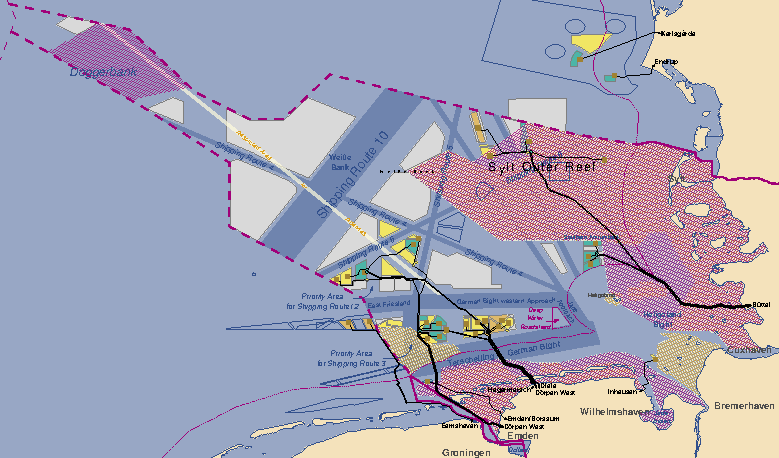
\includegraphics{windfarmplacement/figures/NorthSeaWindFarms.pdf}
    % 
    \caption[The offshore wind farms of the German Bight in the north sea.]{   
        The German offshore wind farms in the North Sea, where the
        \myhl{KITgreen50}{green}, \myhl{KITorange50}{orange}, \myhl{KITyellow50}
        {yellow}, and \myhl{KITblack15}{gray} areas represent wind farms that
        are \myhl{KITgreen50}{operating}, \myhl{KITorange50}{under
        construction}, \myhl{KITyellow50}{approved}, and \myhl{KITblack15}
        {planned}, respectively. There are many restricted zones that are
        prohibited for wind farm planning such as shipping routes, areas
        reserved for gas pipelines, \myhl{KITlilac30}{biota (violet hatched
        area)}, and \myhl{KITorange50}{bird sanctuaries (orange hatched area)}.
        A substation represents roughly speaking a collection point that
        collects the produced energy of wind turbines and forwards it. The
        connections from the last on-water substation to the first substation on
        the land-side (\eg, D{\"o}rpen West, Diele and B{\"u}ttel have
        substations) are usually implemented by~\acrlong{hvdc} (\gls{hvdc}).
        Note that this figure is a modification
        of~\parencite{online:offshore-wind-farm:german-bight}. }%
        % 
    \label{ch:intro:fig:north-sea-wind-farms}
\end{figure}
% 

Long-term power grid configuration has the major disadvantage that the planning
horizon is often in terms of
decades~\parencite{online:europe:TYNDP-2018-Projects-Sheets-166}, which is
counterproductive for the desired plan to change the power grid quickly in the
next few years~\parencite{online:eeg2014}. In addition, each expansion planning
is done for a certain topological scenario meaning a fixed power grid,
generation, and demand configuration. Different scenarios already occur with
different productions and consumptions. Thus, another strategy that covers
different scenarios and different topology changes is the placement of advanced
control units (\cref{ch:intro:strategy:2}). This is known as static design
problem, which is a subproblem of the dynamic design problem. The latter is less
cost intensive and represents a short-term configuration.

For~\cref{ch:intro:strategy:2} devices such as circuit breakers (known
as~\emph{switches}) and~\acrlong{facts} (\gls{facts}) are able to manipulate the
power flow by opening a circuit (switching a transmission line off) or rerouting
a certain fraction of power by changing the susceptance of a transmission line
in a device-specified interval, respectively. Both switches and~\gls{facts} are
able to reduce the generation cost while increasing the power grid operation
limit and satisfying the~$N-1$ criterion~\parencite{LiG13}. The~$N-1$ criterion
is a security and reliability criterion to ensure a stable operation while one
element is removed or has a failure. \textcite{Fis08} mentioned that switching
is already used by~\gls{tso}s in certain cases of emergency to decouple parts of
the grid, avoid abnormal voltage situations, or improve voltage profiles.
However, it is currently not used to extend the operability of the grid or
reduce costs and losses, since the~\gls{tso}s wish to interfere as little as
possible in the power grid to avoid instabilities.

Since power grids are one of the major backbones, their reliability is crucial.
A common and natural belief is that only~\gls{tnep} has the ability to maintain
and improve the reliability and operability of the power grid. However, placing
switches and~\gls{facts} is another way---though counterintuitive---to improve
the efficiency and reliability of the power grid. This counterintuitive behavior
is known as Braess's Paradox~\parencite{Bra68,Bra05} that is a common phenomenon
in many physical networks (see~\cref{ch:related-work:sec:braess-paradox}).
Furthermore, \textcite{Sch90} mentioned that both switches and~\gls{facts} have
the possibility to control over- and under-voltage situations, and line
overloads. Other papers confirm loss and cost reductions~\parencite{Sch90},
system security improvements~\parencite{Sch88}, and combinations of
all~\parencite{Hed11}.

In this work, we mainly focus on~\cref{ch:intro:strategy:2} by placing elements
such as switches or~\gls{facts} in such a way that we increase the operability
of the power grid and thus, the power grid's capacity. Note that increasing the
power grid capacity makes the power grid more reliable. Both electrical elements
can increase the maximum load. Switching provides a possibility to remove a
transmission line from the power grid temporarily. To the contrary, \gls{facts}
are control units that are able to influence the power flow in a certain range.
However,
\gls{facts} are also more expensive and complex. We will look
on~\cref{ch:intro:strategy:1} from the perspective of a plane grid with
generators and consumers, but no preinstalled interconnection. We motivate this
scenario by a wind farm planning problem denoted by wind farm cabling problem.
% 
%%%%%%%%%%%%%%%%%%%%%%%%%%%%%%%%%%%%%%%%%%%%%%%%%%%%%%%%%%%%%%%%%%%%%%%%%%%%%%%%
\section{Main Contributions}
\label{ch:intro:sec:contribution}
%%%%%%%%%%%%%%%%%%%%%%%%%%%%%%%%%%%%%%%%%%%%%%%%%%%%%%%%%%%%%%%%%%%%%%%%%%%%%%%%
% 
The contributions of this thesis are mainly covered by four parts. The first
part is about algorithms and structural results on electrical flows (also known
by the term~\emph{power flows}) and is called the~\acrlong{dc}~\acrlong{feas}.
The following two parts cover an overview of the results that concern the
efficient utilization of the existing power grid by placing switches (\ie,
discrete changes to the power grid) and~\acrlong{facts} (\gls{facts}; \ie,
continuous changes to the power grid), respectively. In the fourth part of this
work, the wind farm cabling results are outlined that
cover~\cref{ch:intro:strategy:1}.
%
%%%%%%%%%%%%%%%%%%%%%%%%%%%%%%%%%%%%%%%%%%%%%%%%%%%%%%%%%%%%%%%%%%%%%%%%%%%%%%%%
\paragraph{The Direct Current Feasibility Problem}
%%%%%%%%%%%%%%%%%%%%%%%%%%%%%%%%%%%%%%%%%%%%%%%%%%%%%%%%%%%%%%%%%%%%%%%%%%%%%%%%
% 
One main tool that we use in this thesis are electrical flows commonly known
under the term power flows. In this part, we will focus on the~\acrlong{dc}
\acrlong{feas} (\gls{dc}~\gls{feas}) that is an approximation of
the~\acrlong{ac}~\acrlong{feas} (\gls{ac}~\gls{feas})
(see~\cref{ch:foundations:sec:power-flow-analyses}). An algorithmic approach to
computing electrical flows will be our first contribution in this thesis and our
most fundamental result. We first give a mathematical description and structural
overview of the problem structure. This description is used to develop
algorithms for the electrical flow. One result shows that electrical flows do
not constitute~\acrlong{tum} (\gls{tum}) bases. However, we show a possible way
to solve the integer~\gls{dc}~\gls{feas}.

The first algorithm for~\gls{dc}~\gls{feas} is based on commonly known reduction
rules that will give us an algorithm that runs
in~$\bigO(\fmagnitude{\vertices}^3)$ time for an~\source-\sink planar power grid
(\ie, a power grid with one generator and one consumer). We give another
algorithmic idea for planar graphs that separates the quadratic relationship of
voltage and current by using two graphs and a mapping of their edges. In
addition to that, we are able to use a geometric interpretation of the problem
to improve the understanding for discrete and continuous changes. Note that for
linear systems the superposition principle holds in the physics and thus,
calculating~\gls{dc}~\gls{feas} for all generator and consumer pairs results in
an electrical flow for the whole power grid.
% 
% However, the last algorithm we
% develop is an efficient algorithm for the power flow calculation that runs
% in~$\bigO(\fmagnitude{\vertices})$ time on~\source-\sink power grid
% and~$\bigO(\fmagnitude{\vertices}^2)$ for general power grids.\franzi{Let's see
% if my intuition is correct}
%
%%%%%%%%%%%%%%%%%%%%%%%%%%%%%%%%%%%%%%%%%%%%%%%%%%%%%%%%%%%%%%%%%%%%%%%%%%%%%%%%
\paragraph{Discrete Changes in Power Grids}
%%%%%%%%%%%%%%%%%%%%%%%%%%%%%%%%%%%%%%%%%%%%%%%%%%%%%%%%%%%%%%%%%%%%%%%%%%%%%%%%
% 
The placement of switches represents a discrete change in the power grid and is
the first placement contribution we will focus on in this work. Note that a
discrete change represents a topology change. In particular, we address a
subproblem of the static design problem called~\acrlong{mtsfp}
(\acrshort{mtsfp}), which we model based on the~\acrshort{dc} electrical flow
(see~\cref{ch:switching:sec:model}). The problem's combinatorial nature makes it
hard to solve~\parencite{Leh14} and the current ways to tackle the problem are
exact but slow methods such as~\acrlong{milp}
(\acrshort{milp})~\parencite{Fis08} or even more complex
models~\parencite{6253283,HAGHIGHAT2015104}, or heuristics without provable
quality guarantees.
%
In contrast, we focus on structural properties and algorithms with provable
performance guarantees for the~\gls{mtsfp}. While it was known that~\gls{mtsfp}
is~\NP-hard in general~\parencite{Leh14}, we show that it is
% 
also~\NP-hard if the network contains only one generator and one consumer  
% 
(\source-\sink-networks). The latter is a generalization of another~\NP-hardness
proof given by~\textcite{Koc16}\footnote{We thank Thomas William Brown for
mentioning the paper of~\textcite{Koc16} to us after the conference talk of our 
paper~\parencite{Gra18}, since this work was not known to us.}.
For~\source-\sink-networks on restricted graph classes (including cacti) we
present an exact algorithm based on~\acrlong{dtp}{s} (\acrshort{dtp}s;
see~\cref{ch:switching:sec:exploit_structural_characteristics:subsec:dtp}).
These paths can be computed on general graphs and form the basis for a new
centrality measure resulting in a new algorithm that works well in practice.
% 
To the best of our knowledge, we are the first to provide an approximation and
an exact algorithm for~\gls{mtsfp} on special graph classes. Simulations on
the~\acrlong{nesta} (\gls{nesta}) benchmark set show that these algorithms
produce near-optimal results on most of the practical instances and thus, much
better solutions compared to the proven guarantee.
% 
%%%%%%%%%%%%%%%%%%%%%%%%%%%%%%%%%%%%%%%%%%%%%%%%%%%%%%%%%%%%%%%%%%%%%%%%%%%%%%%%
\paragraph{Continuous Changes in Power Grids}
%%%%%%%%%%%%%%%%%%%%%%%%%%%%%%%%%%%%%%%%%%%%%%%%%%%%%%%%%%%%%%%%%%%%%%%%%%%%%%%%
% 
Another way to use the grid more efficiently is by placing~\gls{facts}. Contrary
to switches that allow discrete changes, \gls{facts} represent a control unit
that change the electrical flow by scaling the susceptance. This represents
another static design problem and makes use of the existing power grid, too. We
assume that a flow control unit is an \emph{ideal}
\gls{facts}~\parencite{julieGriffin} controlling the electrical flow on its
branch without any restrictions. In the first work, we placed~\gls{facts} on
buses and in the follow-up, we considered ideal~\gls{facts} as elements that can
be only placed on branches. In general, the~\gls{facts} placement was shown to
be~\NP-hard~\parencite{Leh16}. Thus, most of the literature uses exact methods
such as~\acrlong{qp} (\acrshort{qp}) for the general formulation and for
ideal~\gls{facts} we will use an~\gls{milp}.

Using the well-known~\gls{ieee} power systems test
cases~\parencite{online:IEEEtestData,Zimmerman2011a,4075418,Bil70,online:TheUniversityOfEdinburgh:SchoolOfMathematics:PowerSystemsTestCaseArchive,
crow2015computational,Dem77,Gra03,780914,Jos16,6120344,5589973,4113721,Woo13},
we performed simulation experiments related to two key questions, which take
into account that the~\gls{facts} needed for implementing our flow control
vertices in the real power grid constitute a significant and expensive
investment and hence their number should be as small as possible. We investigate
the following two research questions. 
% 
% \crefformat{enumi}{#2\textup{Research Question~#1}#3}
\begin{enumerate}[(Q1)]
    \label{ch:intro:facts:researchQuestion}
    % 
    \item How many ideal~\acrshort{facts} are required and where do they have to
    be placed in order to obtain a lower bound for the operating costs?
    \label{ch:intro:question:numberFacts}
    %
    \item If the number of available ideal~\gls{facts} is given, do we still see
    a positive effect on the operating costs and on the operability of the grid
    during peak periods of the~grid?
    \label{ch:intro:question:costsOperability}
    % \item We consider the state of the grid, where the branch limits are approached
    % and ask whether a limited number of flow control units can decrease the
    % operation costs and extend the grid operability?
    % 
\end{enumerate}
% 
In our simulations we determine the minimum number of flow control units
necessary to achieve the same solution quality as in a power grid in which each
element is controllable and which clearly admits a best bound on what can be
achieved with the network topology. Interestingly, it turns out that a
relatively small number of ideal~\gls{facts} are sufficient for this. In fact,
we can prove a theorem stating a structural graph-theoretic property, which, if
met by the placement of flow control units, implies the optimality of the power
flow and serves as a theoretical explanation of the observed behavior. Research
Question~\ref{ch:intro:question:numberFacts} becomes increasingly relevant as
the consumption of electrical energy grows faster than the grid capacities.
The~\acrlong{opf} (\gls{opf}) minimizes the total generation costs of the power
grid while maintaining a feasible electrical flow. Our experiments indicate that
installing few ideal~\gls{facts} in a power grid is sufficient not only to
achieve lower costs compared to an~\gls{opf} solution, but also allows to
operate the grid at capacities for which no feasible~\gls{opf} solution exists
any more.
% 
%%%%%%%%%%%%%%%%%%%%%%%%%%%%%%%%%%%%%%%%%%%%%%%%%%%%%%%%%%%%%%%%%%%%%%%%%%%%%%%%
\paragraph{Transmission Network Expansion Planning on the Green Field}%
%%%%%%%%%%%%%%%%%%%%%%%%%%%%%%%%%%%%%%%%%%%%%%%%%%%%%%%%%%%%%%%%%%%%%%%%%%%%%%%%
% 
Wind farms are an important and powerful possibility to convert wind into
electricity. There are different challenges that come with the planning of wind
farms such as the placement of turbines, the configuration/profile of turbines
and substations, and the cabling of turbines. The configuration of the whole
farm is computationally too expensive and even the cabling with multiple cable
types is in general~\NP-hard (see~\cref{ch:related-work:sec:wind-farm-cabling}).
To solve this~\NP-hard problem, we use a heuristic approach called Simulated
Annealing (see~\cref{ch:wfcp:sec:simulated-annealing}). We structure the problem
into multiple layers that decrease the overall complexity of the problem. The
problem is decomposed into circuits, substation problem, and full wind farm
cabling problem. We created a first openly available wind farm benchmark set
that is generated randomly and therefore is less structured than the standard
wind farm.
% 
%%%%%%%%%%%%%%%%%%%%%%%%%%%%%%%%%%%%%%%%%%%%%%%%%%%%%%%%%%%%%%%%%%%%%%%%%%%%%%%%
\section{Thesis Outline}
\label{ch:intro:sec:outline}
%%%%%%%%%%%%%%%%%%%%%%%%%%%%%%%%%%%%%%%%%%%%%%%%%%%%%%%%%%%%%%%%%%%%%%%%%%%%%%%%
% 
We give a brief overview of the organization of this thesis. In particular, we
would like to emphasize that parts of this thesis appeared in previously
published proceedings, and reports~\parencite{Lei15b,Lei15,Mch15,Leh17,Gra18}.
% 
\begin{description}
    \item[\cref{ch:related-work}] To understand the state of the art, we give a
    literature overview that is related to our research and differentiate our
    work to the known literature. In the beginning, we give a short summary on
    results concerning (electrical) flows and the development of digital
    techniques to compute such flows. A synergy of techniques known from
    graph-theoretical and power grid analysis is given
    in~\cref{ch:related-work:sec:analyses} that will provide us with techniques
    to understand and analyze power grids. Since our focus is on combinatorial
    problems in power grids, we describe the paradox
    (see~\cref{ch:related-work:sec:braess-paradox}) that makes switching a
    possible way to extend the operability of the power grid. Note that a
    similar effect is observed with~\gls{facts}. We show that there are works
    describing the Braess's Paradox not only for power grids and present known
    theoretical results. As already mentioned, switching increases the
    operability of the power grid. In~\cref{ch:related-work:sec:switching}, we
    give an overview of known techniques to tackle the switching problem and
    show how we classify our work in the current literature. We analyze similar
    things for the~\gls{facts} placement in~\cref{ch:related-work:sec:facts} and
    for the wind farm cabling problem
    in~\cref{ch:related-work:sec:wind-farm-cabling}.
    % 
    \item[\cref{ch:foundations}] In this chapter, we introduce basic terms and
    notions that will be used in this thesis with regards to graph theory
    (see~\cref{ch:foundations:sec:graph-theory}), graph-theoretical flows
    (see~\cref{ch:foundations:sec:graph-theoretical-flows}), and electrical 
    flows (see~\cref{ch:foundations:sec:power-flow-analyses}). For the two
    latter sections, we define the feasibility problems and show the
    relationships between the different models.
    In~\cref{ch:foundations:sec:power-flow-analyses}, we do not only define the
    feasibility problems, but give a broad overview of the models, describe the
    assumptions, advantages and disadvantages of certain model assumptions as
    well as common problems and the complexity of the power flow analysis. 
    % 
    \item[\cref{ch:network-analysis}] To analyze networks, we describe
    that the electrical flow (see~\cref{ch:foundations:sec:power-flow-analyses})
    is a subproblem of many problems that optimize and analyze power grids. In
    the literature overview, we commonly see the usage of the mathematical
    formulation that is solved using a solver such as Gurobi~\parencite{gurobi}.
    However, in this chapter, we analyze the mathematical structure of
    the~\acrlong{dc} \acrlong{feas}. We develop some algorithms for the~\gls{dc}
    electrical flow using the developed structural knowledge of the problem and
    show that the matrices are separately~\acrlong{tum} (\gls{tum}). The whole
    system is not~\gls{tum}. The first algorithm is based on contraction rules
    with worse runtime than solving the system of linear equations of the
    mathematical formulation. Using a reformulation of the electrical flow, we
    are able to design another algorithmic approach that is much simpler.
    % 
    \item[\cref{ch:switching}] This chapter is published in~\parencite{Gra18}.
    Switching is one of the problems that show the existence of Braess's
    Paradox. We classified our work already
    in~\cref{ch:related-work:sec:switching}.
    % 
    % In~\cref{ch:related-work:sec:switching}, we classify our technique in the
    % context of related problems such as~\acrlong{ots} (\gls{ots}) and the
    % existing approaches to tackle this problem. 
    % 
    A fundamental problem definition of~\acrlong{otsp} (\gls{otsp})
    and~\acrlong{mtsfp} (\gls{mtsfp}) is given in~\cref{ch:switching:sec:model}
    describing the relationships between different problems. Several
    transformations of the network model are introduced
    in~\cref{ch:switching:sec:network_modeling}.
    In~\cref{ch:switching:sec:exploit_structural_characteristics}, we describe
    algorithms and structural properties of switching
    % 
    on~\source-\sink-networks as well as showing when it becomes~\NP-hard. A
    2-approximation on special graph structures is provided
    in~\cref{ch:switching:sec:approximation_algorithm_on_cacti}.
    In~\cref{ch:switching:sec:evaluation}, we evaluate our algorithms with
    methodical extensions. We conclude our work
    in~\cref{ch:switching:sec:conclusion} by summarizing the obtained results
    and outline future work including open problems.
    % 
    \item[\cref{ch:facts}] This chapter is published
    in~\parencite{Mch15,Lei15,Lei15b}. Whereas switching represents a discrete
    change in the power grid, \gls{facts} allow a change of the electrical flow
    within an interval by scaling parameters such as the susceptance. Thus, it
    represents another possibility to \textquote{rebalance} the electrical flow
    by changing line parameters that have temporary influence on the topology of
    the power grid. In this chapter, we show that \gls{facts} as well as
    switches are able to increase the operability of the power grid, while
    decreasing the overall generation costs. In addition, we give theoretical
    evidence that certain graph structures provide an optimal electrical flow
    that is equivalent to the min-cost flow.
    % 
    \item[\cref{ch:wfcp}] This chapter is
    published in~\parencite{Leh17}. A fundamental problem definition for the
    wind farm cabling problem is given in~\cref{ch:wfcp:sec:model}, where we
    introduce a first formal hierarchical structure definition of the wind farm
    problem; we further differentiate the full farm problem into the substation
    and circuit problem. The basic simulated annealing algorithm is introduced
    in~\cref{ch:wfcp:sec:simulated-annealing} and we give our methodical
    extensions to this algorithm for the wind farm cabling problem.
    In~\cref{ch:wfcp:sec:sec:simulations}, we evaluate our algorithm by using
    generated graphs as benchmark set. These benchmark sets are often harder
    than the current real world wind farms. We conclude our work
    in~\cref{ch:wfcp:sec:conclusion} by summarizing the obtained results and
    outline future work.
    % 
    \item[\cref{ch:conclusion}] This chapter summarizes the work we have done on
    the previously introduced placement problems in power grids that can
    influence the effect of the Braess's Paradox and thus, are able to improve
    the efficiency of power grids. However, this work is just a start to look at
    these problems from an algorithmic point of view and a lot of further
    investigations are necessary to improve existing algorithms and to
    understand these problems in more detail. Some ideas for possible future
    investigations are outlined in this chapter.
\end{description}
